\documentclass{article}
\usepackage[preprint]{neurips_2026}

\usepackage[utf8]{inputenc}
\usepackage[T1]{fontenc}
\usepackage{hyperref}
\usepackage{url}
\usepackage{booktabs}
\usepackage{amsfonts}
\usepackage{amsmath}
\usepackage{microtype}
\usepackage{xcolor}
\usepackage{graphicx}

% This is an ES 678 course paper, not a conference submission.
\makeatletter
\renewcommand{\@noticestring}{ES 678 Course Project}
\makeatother

\newcommand{\ci}[2]{{\scriptsize[#1, #2]}}

\title{Melanoma Detection from Dermoscopy Images: Lesion-Level Evaluation and Failure-Mode Audit on HAM10000}

\author{%
  Akhil Maan \\
  Roll Number: 25210010 \\
  ES 678 \\
  Indian Institute of Technology Gandhinagar
}

\begin{document}
\maketitle

\begin{abstract}
How well can a classifier separate melanoma from other pigmented lesions in HAM10000 dermoscopy images
when tested only on unseen lesions, how much does a naive image-level split overstate this, and where
do errors concentrate? On a fixed lesion-grouped split, a fine-tuned EfficientNet-B0 reaches a
lesion-level melanoma AUROC of 0.939 [0.921, 0.956], tied with a fine-tuned ResNet-50 and well above a
frozen-feature linear probe (0.852) and a metadata-only model (0.645). A threshold tuned on validation
for 90\% sensitivity gave 79\% on test. On identical test images, a model trained on an image-level
split gains 0.065 AUROC only on lesions whose sibling photos it saw in training, and nothing on unseen
lesions. Errors and over-confidence concentrate in biopsied benign lesions (specificity 0.76, AUROC
0.86), and temperature scaling does not fix subgroup miscalibration. The claim covers this
retrospective two-site dataset only.
\end{abstract}

\section{Problem and Motivation}
Melanoma is curable by excision when found early, so a tool that flags suspicious lesions could help
decide what to biopsy. Reported accuracy on
HAM10000~\citep{tschandl2018} can be inflated: its 10{,}015 images show only 7{,}470 lesions, and
DermaMNIST, a popular benchmark built from it, leaked photos of the same lesion across training and
test sets~\citep{abhishek2025}.
\textbf{Task.} One row is one dermoscopy image. The primary target is melanoma versus all other
diagnoses; the seven-class diagnosis is secondary. A prediction would be made at the clinic visit,
before biopsy, so inputs are the image and, for one baseline, age, sex and body site. How the
diagnosis was confirmed (histopathology, follow-up, consensus, confocal) is known only after the workup
and is tied to the label, so it is never an input and is used only to analyse errors.
\textbf{Claim.} An honest estimate, with uncertainty, of melanoma detection on unseen lesions in this
retrospective two-site dataset, plus an account of where the model fails. It is not a claim of
clinical readiness, and nothing here is causal.

\section{Data and Preparation}
HAM10000 (Harvard Dataverse, CC BY-NC 4.0) holds 600$\times$450 images from the Medical University of
Vienna and a skin cancer practice in Queensland, Australia. Classes are imbalanced: nevi (nv) 6{,}705
images, melanoma (mel) 1{,}113, benign keratosis (bkl) 1{,}099, basal cell carcinoma (bcc) 514,
actinic keratosis (akiec) 327, vascular (vasc) 142, dermatofibroma (df) 115.
\textbf{Quality checks.} 1{,}956 lesions have 2 to 6 photos (4{,}501 images); diagnosis is constant
within every lesion. Age is missing for 57 images and recorded as 0 for 39 more (treated as missing);
sex is unknown for 57 and body site for 234. Confirmation is tied to the label: all melanomas are
histopathology-confirmed, and all 3{,}704 follow-up cases are nevi, nearly all from the Vienna
\textit{molemax} monitoring source. There are no skin-tone labels, and many images show hair, ruler
marks or a dark circular vignette.
\textbf{Splits and preprocessing.} Before any modelling, lesions were split 70/15/15 into train,
validation and test, stratified by diagnosis with a fixed seed (5{,}229 / 1{,}120 / 1{,}121 lesions;
6{,}981 / 1{,}532 / 1{,}502 images; 92 melanoma lesions in test). The split file is saved, and the test
set was scored once per trained model. For the leakage study only, a naive split stratified by image
was also made; 550 of its 1{,}503 test images (37\%) have a sibling photo in its training set. Images
were resized to 224$\times$224 and normalised with fixed ImageNet statistics; flips, 90$^\circ$
rotations and $\pm$10\% brightness, contrast and saturation were applied to training images only.
Age imputation (training median), scaling, one-hot encoding (``unknown'' kept as a level) and class
weights were all fit on training rows only.

\section{Methods}
Let $x$ be an image, $y\in\{1,\dots,K\}$ its diagnosis ($K{=}7$), $f_\theta(x)\in\mathbb{R}^K$ the
logits and $p(x)=\mathrm{softmax}(f_\theta(x))$. The melanoma score is $s(x)=p_{\text{mel}}(x)$; a
lesion's score averages $p$ over its images. Each model adds one step:
\textbf{(i) Majority class}, always nevus, anchors every metric.
\textbf{(ii) Metadata-only}: multinomial logistic regression (L2 with inverse strength $C$, balanced
class weights) on age, sex and body site, showing what is predictable without the image.
\textbf{(iii) Linear probe}: the same regression on frozen 2{,}048-d pooled features of an
ImageNet-pretrained ResNet-50~\citep{he2016}, standardised on training rows.
\textbf{(iv) Fine-tuned CNN}: EfficientNet-B0~\citep{tan2019} (main) and ResNet-50 (alternative), all
layers trained with class-weighted cross-entropy
$\mathcal{L}(\theta)=-\frac{1}{N}\sum_{i=1}^{N} w_{y_i}\log p_{y_i}(x_i)$, $w_k=N/(K N_k)$, where $N$ is
the number of training images and $N_k$ those of class $k$; AdamW (weight decay $10^{-4}$), one-cycle
schedule, 15 epochs, batch 48. Melanoma cues (asymmetry, irregular pigment network, colour variation)
are local colour and texture patterns that pretrained convolutional features capture well, and
transfer learning suits 5{,}229 training lesions; the probe shows whether fine-tuning is worth its
cost. Assumptions: test images share the sites and devices of training images, and most labels are
correct. The optional metadata-plus-image extension was not run.

\section{Evaluation Design}
All tuning used validation data only. For the CNNs I swept the learning rate on seed 0
(EfficientNet-B0: $\{10^{-4}, 3{\cdot}10^{-4}, 10^{-3}\}$, chose $10^{-3}$; ResNet-50:
$\{10^{-4}, 3{\cdot}10^{-4}\}$, chose $10^{-4}$) and kept the epoch with the best lesion-level validation
melanoma AUROC; $C$ was chosen the same way. Augmentation was fixed in advance. Each CNN was trained
with three seeds.
\textbf{Melanoma vs rest:} AUROC, AUPRC, and sensitivity/specificity at threshold $\tau$, the largest
value with validation sensitivity $\geq$90\% (a missed melanoma costs far more than a referral). \textbf{Seven classes:} balanced accuracy (mean per-class recall) and macro-F1, since plain
accuracy rewards predicting nevus. \textbf{Calibration:} Brier score and
$\mathrm{ECE}=\sum_{b=1}^{15}\frac{n_b}{n}\lvert\bar{s}_b-\bar{y}_b\rvert$ over 15 equal-width bins of
$s$ ($n_b$ lesions with mean score $\bar{s}_b$ and melanoma rate $\bar{y}_b$); temperature
scaling~\citep{guo2017} uses $\mathrm{softmax}(f_\theta/T)$ with $T$ minimising validation negative
log-likelihood. \textbf{Uncertainty:} 95\% intervals from 1{,}000 bootstrap resamples of test
\emph{lesions}; for three-seed models each replicate averages the metric over seeds. Metrics are
reported per lesion (main) and per image.

\section{Results and Error Analysis}
\begin{table}[t]
\caption{Lesion-grouped test set, lesion level (1{,}121 lesions, 92 melanomas). Mean over 3 seeds for
CNNs; lesion-bootstrap 95\% CI below. Sens/Spec at the validation-chosen 90\%-sensitivity threshold.}
\label{tab:main}
\centering
\footnotesize
\setlength{\tabcolsep}{3pt}
\begin{tabular}{lcccccccc}
\toprule
Model & AUROC & AUPRC & Sens & Spec & Bal.\ acc & Macro-F1 & Brier & ECE \\
\midrule
Majority class & 0.500 & 0.082 & 0.000 & 1.000 & 0.143 & 0.120 & 0.076 & 0.029 \\
Metadata-only LR & 0.645 & 0.136 & 0.870 & 0.220 & 0.321 & 0.202 & 0.078 & 0.058 \\
 & \ci{.580}{.703} & \ci{.103}{.184} & \ci{.798}{.932} & \ci{.194}{.247} & \ci{.262}{.385} & \ci{.176}{.228} & \ci{.066}{.089} & \ci{.042}{.074} \\
ResNet-50 linear probe & 0.852 & 0.396 & 0.793 & 0.749 & 0.616 & 0.525 & 0.066 & 0.052 \\
 & \ci{.812}{.887} & \ci{.301}{.502} & \ci{.716}{.875} & \ci{.722}{.776} & \ci{.550}{.678} & \ci{.465}{.571} & \ci{.057}{.076} & \ci{.041}{.067} \\
ResNet-50 fine-tuned & 0.940 & 0.642 & 0.837 & 0.878 & 0.785 & 0.727 & 0.058 & 0.051 \\
 & \ci{.919}{.957} & \ci{.548}{.731} & \ci{.769}{.895} & \ci{.860}{.896} & \ci{.739}{.827} & \ci{.676}{.766} & \ci{.049}{.068} & \ci{.043}{.066} \\
EfficientNet-B0 fine-tuned & 0.939 & 0.663 & 0.786 & 0.902 & 0.782 & 0.727 & 0.056 & 0.052 \\
 & \ci{.921}{.956} & \ci{.582}{.739} & \ci{.715}{.853} & \ci{.887}{.918} & \ci{.735}{.829} & \ci{.681}{.765} & \ci{.048}{.065} & \ci{.044}{.065} \\
\bottomrule
\end{tabular}
\vspace{-2mm}
\end{table}

Metadata alone carries a weak signal (Table~\ref{tab:main}; 4\% of images under age 30 are melanoma
against 18\% over 60), and the image adds most of the information. Fine-tuning is clearly worth it:
it beats the linear probe by about 0.09 AUROC and 0.25 AUPRC with non-overlapping intervals, while
EfficientNet-B0 and ResNet-50 are indistinguishable. Seed variation is small for AUROC (SD 0.003 to
0.006) but larger at the operating point (sensitivity SD 0.05 for EfficientNet-B0), because the
threshold rests on about 90 validation melanoma lesions. The key practical result is that \textbf{the
90\% target did not transfer}: test sensitivity was 0.786 \ci{0.715}{0.853}, so 19 of 92 melanomas
were missed (per image: sensitivity 0.836, AUROC 0.918). In the seven-class task, lesion-level recall
was 0.89 nv, 0.80 bcc, 0.79 akiec, 0.73 mel, 0.68 bkl, 0.70 df (11 lesions) and 0.88 vasc (14).

\textbf{Where errors concentrate} (EfficientNet-B0, lesion level, Fig.~\ref{fig:calib}b). Every test
melanoma was biopsied, so sensitivity is only measurable there. False positives concentrate in
biopsied benign lesions: specificity is 0.76 \ci{0.72}{0.79} for histopathology-confirmed
non-melanomas, against 0.91 for consensus and 1.00 for 560 follow-up nevi. Within biopsied lesions
AUROC is 0.86 \ci{0.82}{0.89}, so the headline 0.94 is propped up by easy monitored nevi. Lesions are biopsied
because they look suspicious, so this is an association, not a cause. Sensitivity was 0.74 on the back (28 melanomas) and 0.74 at the Australian practice (AUROC 0.87)
versus 0.84 for the modern Vienna set, with overlapping intervals. The one melanoma under age 30 was
missed, and sensitivity was 0.64 \ci{0.33}{0.90} at 30 to 44 years (11 melanomas); sex showed no clear
difference (0.74 female, 0.83 male). Groups with under 15 melanomas or non-melanomas are flagged as too
small in \texttt{results/subgroup\_audit.csv}.

\textbf{Missed melanomas.} I viewed Grad-CAM~\citep{selvaraju2017} maps (melanoma logit, last
convolutional block, seed 0) for all 19 misses (Fig.~\ref{fig:gradcam}). Every map sits on the
lesion, never on rulers, hair or the vignette, though these appear in several images. Most misses are
small, uniformly dark, fairly symmetric lesions or large pale diffuse ones that resemble nevi or
keratoses: hard cases rather than shortcuts, though Grad-CAM cannot rule out subtler artifact use.

\begin{figure}[t]
\centering
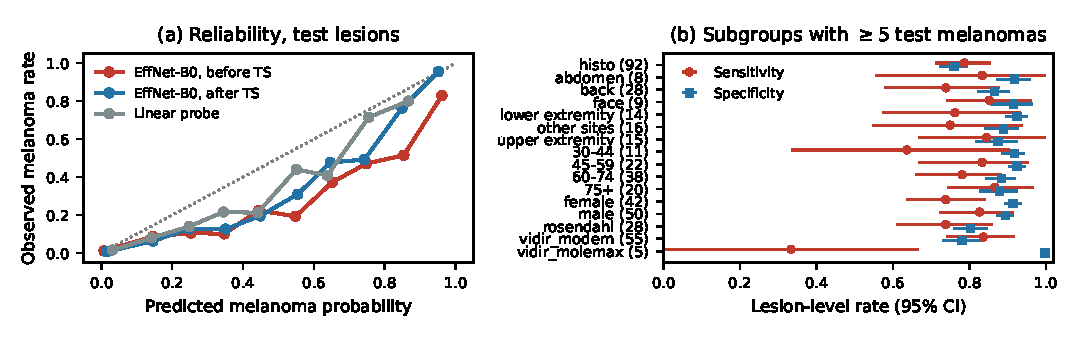
\includegraphics[width=\linewidth]{figures/calibration_subgroups.pdf}
\vspace{-6mm}
\caption{(a) Lesion-level test reliability (bins with $\geq$5 lesions, 3 seeds pooled). (b) Sensitivity
and specificity by confirmation, body site, age, sex and source, with lesion-bootstrap 95\% CIs;
test melanomas in brackets.}
\label{fig:calib}
\vspace{-2mm}
\end{figure}

\section{Graduate Depth Analysis}
\textbf{1. Cost of leakage.} The same EfficientNet-B0 recipe trained on the naive image split looks
better on its own test set (image level): AUROC 0.942 vs 0.918, AUPRC 0.731 vs 0.653, balanced
accuracy 0.817 vs 0.751, sensitivity 0.922 vs 0.836 at similar specificity (0.80); the linear probe
moves the same way (AUROC 0.858 vs 0.823, AUPRC 0.475 vs 0.374). Because these test sets differ, I added
a paired check on \emph{identical} images: the 481 image-split test images whose lesion the
lesion-split model never trained on, grouped by whether the image-split model saw a sibling photo
(Table~\ref{tab:leak}). On unseen lesions the two models are equal; on seen lesions the image-split
model is far better. The difference-in-differences is +0.069 \ci{0.021}{0.123} AUROC and a log-loss
reduction of 0.23 \ci{0.11}{0.35}, so the inflation comes from recognising lesions, not from better
generalisation. Overall the naive split overstated AUROC by 0.02 to 0.04, AUPRC by 0.08 to 0.10 and
balanced accuracy by 0.05 to 0.07; these gaps were never used to choose a model.

\begin{table}[t]
\caption{Paired leakage check on identical image-split test images never trained on by the
lesion-split model (3-seed average). ``Seen'': a sibling photo was in the image-split training set.}
\label{tab:leak}
\centering
\footnotesize
\begin{tabular}{lcccc}
\toprule
& \multicolumn{2}{c}{Seen lesion (188 images, 35 mel)} & \multicolumn{2}{c}{Unseen lesion (293 images, 18 mel)} \\
\cmidrule(lr){2-3}\cmidrule(lr){4-5}
Trained on & Melanoma AUROC & Log-loss & Melanoma AUROC & Log-loss \\
\midrule
Lesion-grouped split & 0.897 \ci{.833}{.949} & 0.70 & 0.954 \ci{.913}{.988} & 0.29 \\
Image-level split & 0.962 \ci{.927}{.987} & 0.48 & 0.950 \ci{.909}{.988} & 0.29 \\
\bottomrule
\end{tabular}
\end{table}

\textbf{2. Error audit:} Section 5 and Fig.~\ref{fig:calib}b. \textbf{3. Calibration.} The fine-tuned CNNs are over-confident: fitted temperatures are 1.38 to 1.60
(EfficientNet-B0) and 1.36 to 1.42 (ResNet-50), and lesions scored near 0.85 were melanoma only about
half the time (Fig.~\ref{fig:calib}a). Temperature scaling lifts that bin to about 0.76 and lowers
image-level ECE from 0.078 to 0.069, but lesion-level ECE is unchanged (0.052 vs 0.053) since
averaging photos already softens scores. It does not fix subgroups: biopsied lesions
have mean predicted probability 0.28 against an observed rate of 0.20 (ECE 0.11, then 0.10), patients
under 30 have ECE 0.17, and in the small Vienna \textit{dias} source (41 lesions) the mean prediction
is 0.37 against 0.10 observed. One global temperature cannot repair group-specific miscalibration, so
scores should not be read as risks.

\begin{figure}[t]
\centering
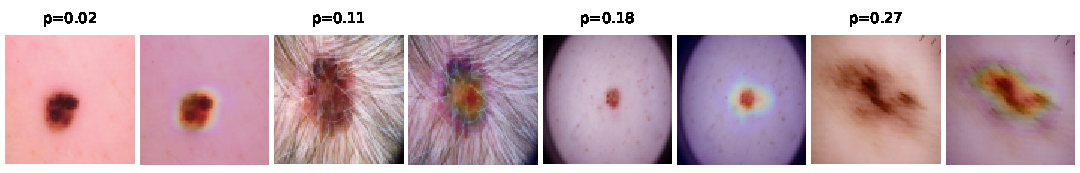
\includegraphics[width=\linewidth]{figures/gradcam_missed.pdf}
\vspace{-6mm}
\caption{Four of the 19 missed test melanomas (image, then Grad-CAM for the melanoma logit;
seed-averaged lesion score $p$, threshold about 0.32). Attention stays on the lesion despite hair,
a vignette and ruler marks.}
\label{fig:gradcam}
\vspace{-3mm}
\end{figure}

\section{Limitations and Conclusion}
The main limitation is scope: images come from a Vienna referral centre and an Australian practice
with heavily sun-damaged patients and carry no skin-tone labels, so nothing here supports claims for
other populations, clinics or devices; a stronger claim needs an external, prospective test set with
consistent histopathology. Also, one fixed split was used (seeds capture training noise, not split
noise), non-biopsied labels may be wrong, and the operating point rests on about 90 validation
melanomas. Results are predictive associations, not causes. \textbf{Answer:} on unseen lesions a
fine-tuned CNN reaches melanoma AUROC about 0.94, but a pre-set threshold gave 0.79 sensitivity instead
of 0.90, and on hard biopsied lesions AUROC falls to 0.86 with over-confidence. A naive image split
inflates scores only through lesions it has already seen.

\section{Reproducibility and AI-Use Disclosure}
Code, split files, per-model predictions, tables and figures:
\url{https://github.com/Akhilmaan616/es678-melanoma-ham10000}. Data come from Harvard Dataverse
(doi:10.7910/DVN/DBW86T) and are not redistributed. \texttt{prepare.py} rebuilds the splits (seed 42);
the README lists the commands that reproduce every number. Training used one RTX 4050 laptop GPU
instead of Colab. No private data or keys are used.
\textbf{AI use:} I used Claude (Anthropic) for brainstorming and for some help with coding. I
checked the code, the split files for lesion overlap, and the reported numbers against the saved
outputs myself.

{\footnotesize
\begin{thebibliography}{9}
\setlength{\itemsep}{0pt}
\bibitem[Tschandl et al.(2018)]{tschandl2018} P.~Tschandl, C.~Rosendahl, and H.~Kittler. The HAM10000 dataset, a large collection of multi-source dermatoscopic images of common pigmented skin lesions. \emph{Scientific Data}, 5:180161, 2018.
\bibitem[Abhishek et al.(2025)]{abhishek2025} K.~Abhishek, A.~Jain, and G.~Hamarneh. Investigating the quality of DermaMNIST and Fitzpatrick17k dermatological image datasets. \emph{Scientific Data}, 12:196, 2025.
\bibitem[Tan and Le(2019)]{tan2019} M.~Tan and Q.~V.~Le. EfficientNet: Rethinking model scaling for convolutional neural networks. In \emph{ICML}, 2019.
\bibitem[He et al.(2016)]{he2016} K.~He, X.~Zhang, S.~Ren, and J.~Sun. Deep residual learning for image recognition. In \emph{CVPR}, 2016.
\bibitem[Guo et al.(2017)]{guo2017} C.~Guo, G.~Pleiss, Y.~Sun, and K.~Q.~Weinberger. On calibration of modern neural networks. In \emph{ICML}, 2017.
\bibitem[Selvaraju et al.(2017)]{selvaraju2017} R.~R.~Selvaraju et al. Grad-CAM: Visual explanations from deep networks via gradient-based localization. In \emph{ICCV}, 2017.
\end{thebibliography}
}

\end{document}
